\documentclass[aspectratio=169,xcolor=table]{beamer}
\usetheme{metropolis}
\usepackage[spanish]{babel}
\usepackage{tikz}
\usetikzlibrary{chains, trees, positioning, shapes}
\usepackage{minted}
\setminted{ style=colorful, fontsize=\small, breaklines}
\usepackage{xcolor-solarized}
\usepackage{fontawesome}
\usepackage{gitdags}
\usepackage{graphicx}
\usepackage{animate}

\newcommand{\twitter}{\href{https://twitter.com/carlosgllp}{\faTwitter\ carlosgllp}}
\newcommand{\github}{\href{https://www.github.com/gpcarlos}{\faGithub\ gpcarlos}}
\newcommand{\warnning}{{\color{solarized-red}\faWarning}}

\title{Introducción a Git y GitHub}
\subtitle{ }
\author{Carlos Gallardo Polanco \\ \twitter \\ \github}
% \institute{Escuela Superior de Ingeniería}
\date{22 de mayo de 2018}
\subject{Betabeers}
\keywords{Git, GitHub, LaTeX}

\definecolor{fafafa}{rgb}{0.98, 0.98, 0.98}
\newcommand{\whiteTitle}{
  \title{\color{fafafa}Introducción a Git y GitHub}
  \author{\color{fafafa}Carlos Gallardo Polanco \\ \twitter \\ \github}
  % \institute{\color{fafafa}Escuela Superior de Ingeniería}
  \date{\color{fafafa}22 de mayo de 2018}
}

% ================================================
% ================================================
% ================================================

\begin{document}

\begin{frame}
  \maketitle
  \begin{tikzpicture}[remember picture,overlay]
    \node[anchor=north east,inner sep=40pt] at (current page.north east) {
\includegraphics[scale=0.065]{images/logoGit.png}};
    \node[anchor=south east,inner sep=40pt] at (current page.south east) {
\includegraphics[scale=0.11]{images/logoBetabeers.png}};
  \end{tikzpicture}
\end{frame}

%  Introducción
\begin{frame}{¿Qué es Git?}
  \begin{columns}[onlytextwidth]
    \column{0.5\textwidth}
    \begin{center}
      
\includegraphics[scale=0.07]{images/logoGit2}
    \end{center}
    \column{0.5\textwidth}
    Git es un Sistema de Control de Versiones (VCS) que nos permite gestionar los cambios que realizamos un proyecto.
  \end{columns}
\end{frame}

\begin{frame}{¿Qué es Git?}
  \begin{columns}[onlytextwidth]
    \column{0.5\textwidth}
    \alert{\Large ¿Git = GitHub? {\color{solarized-red} \textbf{No}}} \\
    GitHub es una forja (plataforma de desarrollo colaborativo) para alojar proyectos Git.
    \column{0.5\textwidth}
    \begin{center}
      \animategraphics[height=1.3in,autoplay,loop] {12}{images/DF/githubDP1_}{0}{7}
      \animategraphics[height=1.3in,autoplay,loop] {12}{images/DF/githubDP2_}{0}{13}
    \end{center}
  \end{columns}
\end{frame}

\begin{frame}{¿Qué es Git?}
  \alert{\Large ¿Cómo se utiliza Git?}
  \begin{columns}[onlytextwidth]
    \column{0.6\textwidth}
    Git se utiliza mediante comandos en la \textbf{Terminal}. \\

    Pero existen:
    \begin{itemize}
      \item Clientes gráficos (GitKraken, SourceTree, GitHub Desktop...)
      \item Integración en muchos editores e IDEs (Atom, Visual Studio Code, Eclipse...)
    \end{itemize}
    \vspace{0.5cm}
    \uncover<2>{
    {\color{violet}\large Lo mejor es la \textbf{Terminal}.}}
    \column{0.4\textwidth}
    \uncover<2>{
    
\includegraphics[scale=0.4]{images/hackerMan.eps}}
  \end{columns}
\end{frame}


%  Conceptos básicos
\begin{frame}[fragile]{Comandos básicos - Iniciar un repositorio}
  \begin{columns}[onlytextwidth]
    \column{0.6\textwidth}
    \alert{Inicializar un repositorio}
    \begin{minted}{console}
    $ git init
    \end{minted}

    \alert{Clonar un repositorio de un remoto (\faGithubAlt GitHub!)}
    \begin{minted}{console}
    $ git clone <url>
    \end{minted}
    \column{0.4\textwidth}
    \tikzstyle{every node}=[draw=solarized-base1,thick,anchor=west]
    \tikzstyle{selected}=[draw=solarized-green,fill=solarized-green!30]
    \begin{tikzpicture}[%
      grow via three points={one child at (0.5,-0.7) and
      two children at (0.5,-0.7) and (0.5,-1.4)},
      edge from parent path={(\tikzparentnode.south) |- (\tikzchildnode.west)}]
      \node {directory}
        child { node [selected] {.git}}
        child { node {source}}
        child { node {LICENSE}}
        child { node {README.md}};
    \end{tikzpicture}
  \end{columns}
\end{frame}

\begin{frame}[fragile]{Comandos básicos - Preparar y confirmar}
  \alert{Añadir un archivo al área de preparación}
  \begin{minted}{console}
    $ git add <archivo>
  \end{minted}

  \alert{Confirmar los cambios}
  \begin{minted}{console}
    $ git commit
    $ git commit -m 'mensaje'
  \end{minted}

  \alert{Saltarse el área de preparación}
  \begin{minted}{console}
    $ git commit -a -m 'mensaje'
  \end{minted}
  \hspace{1cm} {\scriptsize Sólo prepara y confirma los archivos que Git está rastreando!}

  \begin{tikzpicture}[remember picture,overlay]
    \node[anchor=north east, inner xsep=45pt, inner ysep=60pt] at (current page.north east) {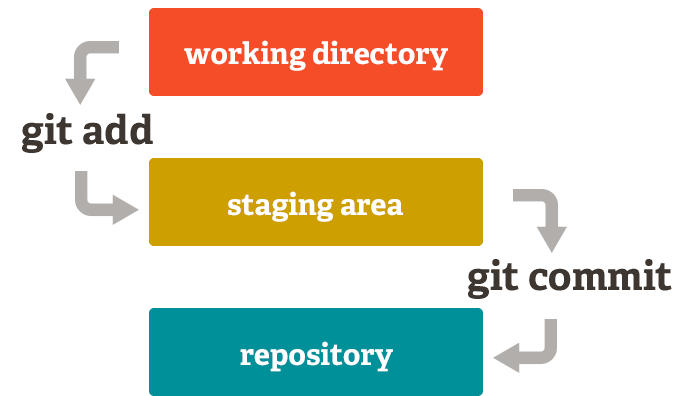
\includegraphics[scale=0.2]{images/areas}};
  \end{tikzpicture}
\end{frame}

\begin{frame}[fragile]{Comandos básicos - Revisar el estado}
  \begin{columns}[onlytextwidth]
  \column{0.35\textwidth}
  Diferencia entre archivos preparados, no preparados pero rastreados y no rastreados.
  \begin{minted}{console}
    $ git status
    $ git status -s
  \end{minted}
  \column{0.02\textwidth}
  \column{0.63\textwidth}
  \vspace{0.3cm}
  \begin{minted}[escapeinside=||, frame=single, framerule=1pt, fontsize=\scriptsize, bgcolor=solarized-base1!30]{console}
[user@linux ~]$ git status
On branch master
Changes to be committed:
(use "git reset HEAD <file>..." to unstage)
|  {\color{solarized-green}new file:   presentation.tex}|
|  {\color{solarized-green}deleted:    basura.text}|
Changes not staged for commit:
(use "git add <file>..." to update what will be committed)
(use "git checkout -- <file>..." to discard changes in working directory)
|  {\color{solarized-red}modified:   .gitignore}|
Untracked files:
(use "git add <file>..." to include in what will be committed)
|  {\color{solarized-red}configuration.tex}|
  \end{minted}
  \end{columns}
\end{frame}

% \begin{frame}[fragile]{Comandos básicos - Revisar el estado}
%   \begin{columns}[onlytextwidth]
%   \column{0.35\textwidth}
%   \begin{tabular}{rcl}
%     \texttt{A} & $\Rightarrow$ & Nuevo \\
%     \texttt{M} & $\Rightarrow$ & Modificado \\
%     \texttt{D} & $\Rightarrow$ & Eliminado \\
%     \texttt{?} & $\Rightarrow$ & No rastreado \\
%   \end{tabular}
%   \column{0.02\textwidth}
%   \column{0.63\textwidth}
%   \begin{minted}[escapeinside=||, frame=single, framerule=1pt, fontsize=\scriptsize, bgcolor=solarized-base1!30]{console}
% [user@linux ~]$ git status -s
% | {\color{solarized-red}M}| .gitignore
% |{\color{solarized-green}D} | basura.text
% |{\color{solarized-green}A} | presentation.tex
% |{\color{solarized-red}??}| configuration.tex
%   \end{minted}
%   \begin{center}
%   $1^a$ columna: En estado preparado \\
%   $2^a$ columna: En estado no preparado
%   \end{center}
%   \end{columns}
% \end{frame}

\begin{frame}[fragile]{Comandos básicos - Eliminar y Renombrar}
  \alert{Eliminar}
  \begin{itemize}
    \item Eliminar un archivo no preparado \warnning
    \begin{minted}{console}
  $ git rm <archivo>
    \end{minted}
    \item Eliminar un archivo preparado \warnning
    \begin{minted}{console}
  $ git rm -f <archivo>
    \end{minted}
    \item Eliminar del repositorio pero no del directorio de trabajo
    \begin{minted}{console}
  $ git rm --cached <archivo>
    \end{minted}
  \end{itemize}

  \alert{Renombrar}
  \begin{minted}{console}
    $ git mv <archivo> <archivo-nuevo>
  \end{minted}

\end{frame}


%  Remotos (pull y push)
\begin{frame}{Trabajar con Remotos}
  \begin{itemize}
    \item \alert{Ver tus remotos}
      \mint{console}| $ git remote -v|
    \item \alert{Añadir un remoto}
      \mint{console}| $ git remote add <nombre-remoto> <url>|
    \item \alert{Inspeccionar un remoto}
      \mint{console}| $ git remote show <nombre-remoto>|
    \item \alert{Eliminar un remoto}
      \mint{console}| $ git remote rm <nombre-remoto>|
    \item \alert{Renombrar un remoto}
      \mint{console}| $ git remote rename <nombre> <nombre-nuevo>|
  \end{itemize}
\end{frame}

\begin{frame}{Trabajar con Remotos}
  \begin{itemize}
    \item \alert{Traer remotos}
      \mint{console}| $ git fetch <nombre-remoto>|
      {\scriptsize Creará una nueva rama con el trabajo del remoto}
    \item \alert{Traer y Combinar remotos}
      \mint{console}| $ git pull <nombre-remoto> <nombre-rama>|
      \texttt{push = fetch + merge}
    \item \alert{Enviar a tus remotos}
      \mint{console}| $ git push <nombre-remoto> <nombre-rama>|
  \end{itemize}
  Si nuestra rama sigue a la rama remota, se puede no especificar nombres
  \begin{tikzpicture}[remember picture,overlay]
    \node[anchor=north east,inner ysep=50pt, inner xsep=20pt] at (current page.north east) {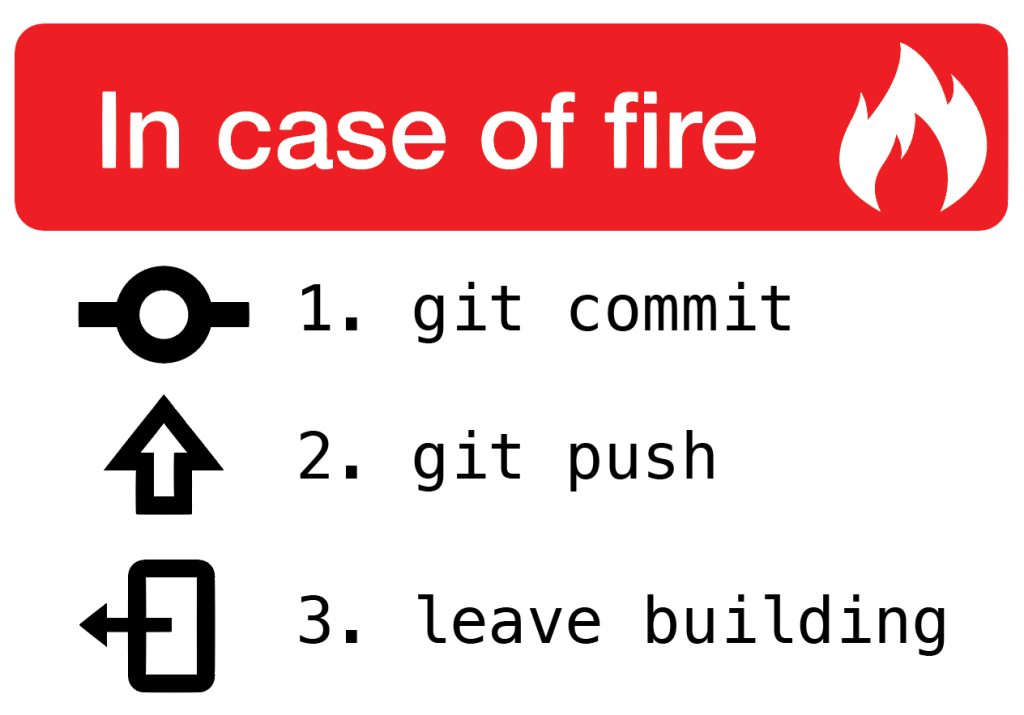
\includegraphics[scale=0.5]{images/incaseoffire.png}};
  \end{tikzpicture}
\end{frame}

\begin{frame}{Trabajar con Remotos - Seguimiento}
  \begin{itemize}
    \item \alert{Crear una rama de seguimiento}
      \mint{console}| $ git checkout --track <remoto>/<rama>|
      {\scriptsize La rama se llamará \texttt{<rama>} y nos moveremos a ella}
      \mint{console}| $ git checkout -b <rama> <remoto>/<rama>|
    \item \alert{Asignar seguimiento a una rama creada}
      \mint{console}| $ git branch -u <remoto>/<rama>|
    \item \alert{Ver las ramas a la que hace seguimiento}
      \mint{console}| $ git branch -vv|
  \end{itemize}
  Cuando hacemos \texttt{clone}, automáticamente \texttt{master} hace seguimiento de \texttt{origin/master}
\end{frame}


\section{Ejemplo}

%  githubEducation
\begin{frame}{GitHub Education}
  \begin{center}
  \begin{figure}
    
\includegraphics[scale=0.2]{images/githubEducation}
  \end{figure}
  \href{https://education.github.com}{\Large{education.github.com}}
  \end{center}

\end{frame}


%  GitStats y Gource
\begin{frame}{Estadísticas y visualización}
  \begin{columns}[onlytextwidth]
    \column{0.4\textwidth}
      
\includegraphics[scale=0.23]{images/analysis}
    \column{0.6\textwidth}
    \begin{itemize}
      \item[] \href{http://gource.io}{\Large{gource.io}}
      \item[]
      \item[] \href{http://gitstats.sourceforge.net}{\Large{gitstats.sourceforge.net}}
    \end{itemize}
  \end{columns}
\end{frame}


\begin{frame}{Bibliografía}
  \nocite{*}
  \bibliography{bibliography}
  \bibliographystyle{plain}
\end{frame}

\begin{frame}[standout]
  \whiteTitle
  \maketitle
  \begin{tikzpicture}[remember picture,overlay]
    \node[anchor=north east,inner sep=40pt] at (current page.north east) {
\includegraphics[scale=0.27]{images/logoGitw.png}};
    \node[anchor=south east,inner sep=40pt] at (current page.south east) {
\includegraphics[scale=0.11]{images/logoBetabeersw.png}};
  \end{tikzpicture}
\end{frame}

\end{document}
